\documentclass[12pt, a4paper]{article}
\usepackage{caption}
\usepackage{graphicx}
\usepackage{hyperref}
\hypersetup{
    colorlinks,
    citecolor=black,
    filecolor=black,
    linkcolor=black,
    urlcolor=black
}
\usepackage{tikz-network}
\usepackage{amsmath, amsfonts, amssymb, amsthm}
\usepackage{algpseudocode}
\usepackage{algorithm}
\title{Database management \\and database systems}
\date{2022}
\author{Kristoffer Klokker}

\usepackage{xcolor,listings}
\usepackage{textcomp}
\usepackage{color}
\usepackage{listings}
\definecolor{codegreen}{rgb}{0,0.6,0}
\definecolor{codegray}{rgb}{0.5,0.5,0.5}
\definecolor{codepurple}{HTML}{C42043}
\definecolor{backcolour}{HTML}{F2F2F2}
\definecolor{bookColor}{cmyk}{0,0,0,0.90}  
\color{bookColor}

\lstset{upquote=true}

\lstdefinestyle{mystyle}{
    backgroundcolor=\color{backcolour},   
    commentstyle=\color{codegreen},
    keywordstyle=\color{codepurple},
    numberstyle=\numberstyle,
    stringstyle=\color{codepurple},
    basicstyle=\footnotesize\ttfamily,
    breakatwhitespace=false,
    breaklines=true,
    captionpos=b,
    keepspaces=true,
    numbers=left,
    numbersep=10pt,
    showspaces=false,
    showstringspaces=false,
    showtabs=false,
    tabsize=3,
}
\lstset{style=mystyle}
\usepackage{zref-base}

\makeatletter
\newcounter{mylstlisting}
\newcounter{mylstlines}
\lst@AddToHook{PreSet}{%
  \stepcounter{mylstlisting}%
  \ifnum\mylstlines=1\relax
    \lstset{numbers=none}
  \else
    \lstset{numbers=left}
  \fi
  \setcounter{mylstlines}{0}%
}
\lst@AddToHook{EveryPar}{%
  \stepcounter{mylstlines}%
}
\lst@AddToHook{ExitVars}{%
  \begingroup
    \zref@wrapper@immediate{%
      \zref@setcurrent{default}{\the\value{mylstlines}}%
      \zref@labelbyprops{mylstlines\the\value{mylstlisting}}{default}%
    }%
  \endgroup
}

% \mylstlines print number of lines inside listing caption
\newcommand*{\mylstlines}{%
  \zref@extractdefault{mylstlines\the\value{mylstlisting}}{default}{0}%
}
\makeatother


\newcommand\numberstyle[1]{%
    \footnotesize
    \color{codegray}%
    \ttfamily
    \ifnum#1<10 0\fi#1 |%
}

\newcommand{\beginSQL}{\begin{lstlisting}[ language=SQL,
                    deletekeywords={IDENTITY},
                    deletekeywords={[2]INT},
                    morekeywords={clustered},
                    framesep=8pt,
                    xleftmargin=40pt,
                    framexleftmargin=40pt,
                    frame=tb,
                    framerule=0pt ]}

\def\ojoin{\setbox0=\hbox{$\bowtie$}%
  \rule[-.02ex]{.25em}{.4pt}\llap{\rule[\ht0]{.25em}{.4pt}}}
\def\leftouterjoin{\mathbin{\ojoin\mkern-5.8mu\bowtie}}
\def\rightouterjoin{\mathbin{\bowtie\mkern-5.8mu\ojoin}}
\def\fullouterjoin{\mathbin{\ojoin\mkern-5.8mu\bowtie\mkern-5.8mu\ojoin}}
\begin{document}
	\maketitle
	\clearpage
	\tableofcontents
	\clearpage
	\section{Database introduction}
		Databases are a collection of data stored in a DBMS (database management system) which serves the purpose of:
			\begin{itemize}
				\item Create database and specifying their schemas (logical structure of the data)
				\item Query the data (questions about data or retrieving the data)
				\item Store large amount of data in long periods with easy access and modificatio of the data
				\item Durable and should be able to recover data in case of error or misuse
				\item Allow multiple user access at once
			\end{itemize}
			Today the norm in database systems are relation databasese which present the data as tables, and the underlying datastructure is not needed for use of the system.\\
			In the case of multiple different database and systems which should be syncronised either a data warehouse is used where a periodically copy of the smaller databases is made. Another approach is a middleware which is a translation between two databases schemes.\\
			A database has mainly two users, admin which can modify the schema using DDL command (data-definition language) which modify the schema by altering the metadata.\\
			The other user being a normal user allowed to do DML command (data-manipulation language). \\
			When a DML command is executed two subsystems are handling the command:
				\subsection{Query compiler}
					The compiler takes the query and creates a query plan (a sequence of actions) and passes it the the execution engine.\\
					A request of data sends data data in tuples to the buffer manager, which is responsible for all data transaction between disk storage and memory\\
					The compiler consist of
					\begin{itemize}
						\item Query parser - which builds a tree from the textual query
						\item Query preprocessor - Sematic check of query to ensure a valid query and transforms the query into algebraic operators
						\item Query optimizer - Transofrm the query to the best avaliable sequence of operation on the actual data based on metadata and schema structure
					\end{itemize}
				\subsection{Transaction manager}
					The transaction manager is used to log for possible recovering and ensuring durablity\\
					Also the transaction has a concurrency-controle manager to ensure a bundle of transaction is executed as they were one unit and locking data when used to ensure no data is wrongly overwritten.\\
					The transaction also manages such that every execution is isolated in case of revertion.\\
					The transaction followed the ACID test, where
					\begin{itemize}
						\item A - atomicity which ensures that in case of error a transaction is never half completed
						\item C - consistency in data and data constraints
						\item I - isolation ofe ach operation done in order in a transaction
						\item D - durability of data such it is never lost after a transaction
					\end{itemize}
	\section{The relational model of data}
		A data model is used for describing data and conisist of:
		\begin{itemize}
			\item Structure of data - Referred to as physical data model, but is simply a high level data structure
			\item Operations on the data - A limited set of operations in DBS at hight level, which makes it more flexible for underlying improvements
			\item Constraints of data - Constraints on data to ensure data integrity
		\end{itemize} 
		\subsection{The semistructured-data model}
			The data is setup in a relation more like a tree rather than table.\\
			Here XML is mostly used to represent datam by nested tags.
			\begin{lstlisting}
<Movies>
	<Movie title="Gone with the wind">
		<Year>1939</Year>
		<Length>231</Length>
		<Genre>drama</Genre>
	</Movie>
	<Movie title="Star Wars">
		<Year>1977</Year>
		<Length>124</Length>
		<Genre>sciFi</Genre>
	</Movie>
</Movies>
			\end{lstlisting}
		\subsection{Document Type Definition model}
			This is model based on XML to standify a more text based model of a database. This model focus on all the data types in a database and how they are nested.
			An example is as follows:
			\begin{lstlisting}            
<!DOCTYPE Stars [
	<!ELEMENT Stars (Star*)>
	<!ELEMENT Star (Name, Address+, Movie*)>
	<!ELEMENT Name (#PCDATA)>
	<!ELEMENT ADDRESS (Street, City)>
	<!ELEMENT Street (#PCDATA)>
	<!ELEMENT CITY (#PCDATA)>
	<!ELEMENT Movie EMPTY>
		<!ATLIST Title CDATA #REQUIRED, Genre CDATA #IMPLIED>
]>
		\end{lstlisting}
		Here $\#PCDATA$ is some data for an element and it can here be seen how nesting is allowed by defining star with address wich is also defined later.\\
		Here the database Stars also include any number of star as stated at first.\\
		The last movie is an alternative writing were instead of $<Movie>Hello</Movie>$ the $EMPTY$ makes it be $<Movie Title="Hello", "Comedy">$, $CDATA$ is simply characterData and $\#REQUIRED$ means it must be filled whereas $\#IMPLIED$ is optional.
		\subsection{The basics of relational database}
			Relation refers to the two dimensional table of data.With attributes being the coloumns and rows being a tuple. The tuple is then made of an relations where a relation with attributes are a schema. \\
			A relation is defined by $Name(attribute:type, attribute2: type)$ and a tuple is in the same order and valeis for the given attributes.\\
			Relations comes in sets and not lists and therefore order is not important\\
			A database may contain a key which is attribute(s) which define a unique relation, if no combination of attributes are unique a ID for the relation can be created.\\
		\subsection{SQL language}
			SQL is the language used to create queries. SQL has tree kinds of relations, stored called tables (relations), views (relation which are not stored but used for computation), temporary tables (tables constructed by SQL temporary)\\
			The data types avaliable by SQL are:
			\begin{itemize}
				\item $CHAR(n)$ - Character string of fixed length $n$
				\item $BIT$ - Logical value with possible values being TRUE, FALSE, UNKNOWN
				\item $INT$ - Number can also be $SHORTINT$ for small number
				\item $FLOAT$ - Higher precision numbers here $DOUBLE$ can also be used for more precision
				\item $DECIMAL(n,d)$ - Numbers of length $n$ and the decinam placed at $d$
				\item $DATE$ and $TIME$ - both essentially being strings with a strict format
			\end{itemize}
			The basic commands for modifying tables are:
			\begin{itemize}
				\item DROP TABLE R; which removes the table $R$ with all its entries
				\item ALTER TABLE R ADD a type; Adds attribute $a$ as a $type$ to table $R$
				\item ALTER TALBE R DROP a; Removes the attribute $a$ form table $R$
			\end{itemize}
			SQL also has $DEFAULT$ which can be added after any attribute after type and describes the default value if non is given.\\
			\subsubsection{Keys}
				A PRIMARY KEY is used for securing no dublicates and only allows non null values in the key attribute.\\
				UNIQUE allows null as a value in its attribute, but dublicates is still nto allowed.\\
				When creating a table the key can be choosen by after an attribute after its type $PRIMARY\; KEY$ or $UNIQUE$ is inserted or at the end of the table definition $PRIMARY\; KEY\; (a)$ can be inserted where a are the attributes. Again Unique can also be used like this.
	\section{Algebraic Query Language}
		The algebraic query langauge is the operation behind the SQL real language.\\
		This is not a programming language, but the simplicity makes in easier to optimize and faster.\\
		All the operations works on boths sets and bags(the allowance of mutliple accourences of tuples)\\
		The following table is in precedence order from first at top and last on bottom.\\
		\begin{table}[h!]
		\begin{tabular}{|l|l|l|l|}
		\hline
		Name       & Symbol               & Effect                                                                                                      & * \\ \hline
		Selection  & $\sigma_C(R)$         & Select tuples from R which meets the condition $C$                                                          &             \\ \hline
		Projection & $\pi_{A1,A2}(R)$     & All tuples from R but only attributes $A1$ and $A2$                                                         &        4     \\ \hline
		Rename     & $\rho_{S(A1,A2)}(R)$ & \begin{tabular}[c]{@{}l@{}}All tuples in R but rename attributes to A1 and A2\\ Alternative $R2_{A1,A2}:=R$\end{tabular}   & \\ \hline
		Duplicate Elem.  & $\delta (R)$            & Eliminate dublicate tubles in relation R                                                                            &            \\ \hline
		Aggregation  & Ex. $SUM(B)$            & Computes operation on given attribute B                                                                           &         3   \\ \hline
		Group  & $\gamma_{B,SUM(C)\rightarrow s}R $   &\begin{tabular}[c]{@{}l@{}}Group relation R by attribute B and in this\\ example creates attribute s with the sum of\\ attribute C to each goup\end{tabular}                                                &            \\ \hline
		Sort  & $\tau_{A1,A2}(R) $   &Sort relation R according to A1 and A2 &            \\ \hline
		Cartesian  & $R\times S$          & Every possible combination of tuples from R and S                                                           & 2           \\ \hline
		Nat. join  & $R\bowtie S$         & \begin{tabular}[c]{@{}l@{}}Cartesian product but only\\ where overlapping attributes are equal\end{tabular} & 2           \\ \hline
		Theta join & $R\bowtie_CS$        & \begin{tabular}[c]{@{}l@{}}Every cartesian product of R and S\\ which meet the $C$ condition\end{tabular}   & 2           \\ \hline
		Outer join & $R \fullouterjoin S$ & \begin{tabular}[c]{@{}l@{}}Nat. join but none joined tubles, are padded\\ with NULL/$\bot$. Also in variations\\ of $\leftouterjoin$ where only all tubles from R is kept,\\ and $\rightouterjoin$ which keep all from S \end{tabular}  &            \\ \hline
		Difference & $R- S$               & Tuples which in R which is not in S                                                                         & 1           \\ \hline		
		Union      & $R\cup S$            & All tuples from R and S                                                                                     & 1           \\ \hline
		Intersect  & $R\cap S$            & Tuples which are in both R and S                                                                            & 1           \\ \hline
		\end{tabular}
		\end{table}
		\begin{enumerate}
			\item Same attributes (and same type) in same order
			\item In case of attributes with same name they will be "renamed" to 'relationName.Attribute'
			\item The standard aggreagation operations are: SUM,AVG,MIN,MAX,COUNT
			\item Attribute A1 can also be 'A1 $rightarrow$ k' for renaming it to, or some expression like 'A1 + A2 $\rightarrow$ sum'
		\end{enumerate}
		It can here be seen that there is multiple combinations which are equal. Here the highest priority readability due to the query compiler rewriting it anyway.\\
		When writing linear notation be used as such:
		$$R(a,y,l):=\sigma_{age<18}(People)$$
		From which $R$ now can be usedas a variable.\\
		Often when combining operationsa tree is used where root is the final product and branches are the first operations done.
		\subsection{Examples}
			\begin{minipage}[t]{0.32\textwidth}
				\begin{center}
				$A$\\
				\begin{tabular}{|l|l|}
				\hline
				A & B \\ \hline
				1 & 5 \\ \hline
				2 & 4 \\ \hline
				\end{tabular}\\[4mm]
				$A\cup C$\\
				\begin{tabular}{|l|l|}
				\hline
				A & B \\ \hline
				1 & 5 \\ \hline
				2 & 4 \\ \hline
				1 & 5 \\ \hline
				7 & 0 \\ \hline
				\end{tabular}\\[4mm]
				$\sigma_{B<4}(C)$\\
				\begin{tabular}{|l|l|}
				\hline
				A & B \\ \hline
				7 & 0 \\ \hline
				\end{tabular}\\[4mm]
				$A\bowtie B$\\
				\begin{tabular}{|l|l|l|}
				\hline
				 A & B & C \\ \hline
				 1 & 5 & 8 \\ \hline
				 2 & 4 & 9 \\ \hline
				\end{tabular}
				
				\end{center}
			\end{minipage}
			\begin{minipage}[t]{0.32\textwidth}
				\begin{center}
				$B$\\
				\begin{tabular}{|l|l|}
				\hline
				B & C \\ \hline
				5 & 8 \\ \hline
				4 & 9 \\ \hline
				\end{tabular}\\[4mm]
				$A\cap C$\\
				\begin{tabular}{|l|l|}
				\hline
				A & B \\ \hline
				1 & 5 \\ \hline
				\end{tabular}\\[4mm]
				$\pi_B(A)$\\
				\begin{tabular}{|l|}
				\hline
				 B \\ \hline
				 5 \\ \hline
				 4 \\ \hline
				\end{tabular}\\[4mm]
				$A\bowtie_{A.B = B.B}C$\\
				\begin{tabular}{|l|l|l|l|}
				\hline
				A & A.B & B.B & C \\ \hline
				1 & 5 & 5 & 8\\ \hline
				2 & 4 & 4 & 9\\ \hline
				\end{tabular}
				\end{center}				
			\end{minipage}
			\begin{minipage}[t]{0.32\textwidth}
				\begin{center}
				$C$\\
				\begin{tabular}{|l|l|}
				\hline
				A & B \\ \hline
				1 & 5 \\ \hline
				7 & 0 \\ \hline
				\end{tabular}\\[4mm]
				$A- C$\\
				\begin{tabular}{|l|l|}
				\hline
				A & B \\ \hline
				2 & 4 \\ \hline
				\end{tabular}\\[4mm]
				$A\times B$\\
				\begin{tabular}{|l|l|l|l|}
				\hline
				A & A.B & B.B & C \\ \hline
				1 & 5 & 5 & 8\\ \hline
				1 & 5 & 4 & 9\\ \hline
				2 & 4 & 5 & 8\\ \hline
				2 & 4 & 4 & 9\\ \hline
				\end{tabular}\\[4mm]
				$\rho_{G,K}(A)$\\
				\begin{tabular}{|l|l|}
				\hline
				G & K \\ \hline
				1 & 5 \\ \hline
				2 & 4 \\ \hline
				\end{tabular}
				\end{center}				
			\end{minipage}
	\section{Queries in SQL}
		\subsection{Select}
			The most simple query is the SELECT FROM WHERE.\\
			This a simple select query which selects attributes from a database where a conditions is met.\\
			The conditions can use the 6 comparisions operators: $=,<>,<,>,<=,>=$ where $<>$ is not equal.\\
			Operations may also be done on values for int $+,-,*,/,\%$ and for string $||$ which adds two string together.\\
			When comparing string the $<$ operators are defined upon lexicongraphic order.\\
			For string the LIKE can be used to match a pattern. A pattern uses $\%$ and $\_$ where $\%$ is any number of wildcard charachters and $\_$ is a single charachter.\\
			Strings are defined by ' therefore when working with them inside a string two ' is used like ''\\
			Logic operators avaliable is AND, OR and NOT\\
			Ex. SELECT title, genre FROM Books WHERE author = Kristoffer Klokker AND year = 2022\\
		\subsection{Default}
			When creating a realtion, the default attribute can be used in case of a not given value.\\
			CREATE TABLE CoolPeople(name CHAR(30) DEFAULT 'Kristoffer Klokker', phone CHAR(16));
		\subsection{Modifying the database}
			\subsubsection{Insert}
				INSERT INTO R VALUES (A1,A2..)\\
				Insert a tuble into relation R with values A1, A2 as the attributes in same order.\\
				Alternative INSERT INTO R(Sum,Name) VALUES (A1,A2..), which will insert the value to the corresponding attrubute.\\
				A1 and A2 can also be a tubles by itself from another DB, for inserting multiple tubles at once.
			\subsubsection{Deletion}
				DELETE FROM R WHERE <condition>\\
				Delete every tuple in relation R which satifies the condition.\\
				Remember deletion is not a linear process rather all satifiable tuples will be deleted once all are found.
			\subsection{Update}
				UPDATE R SET name = 'Kristofer' WHERE <condition>\\
				Changes attribute value, where the condition is met.
		\subsection{Rename}
			In case of a rename of attributes the keywords AS is used, here it is also possible to modify values.\\
			Ex. SELECT title + ' and the stone' AS name from Books\\
			COnstants are also avaliable if wanted.\\
			Ex. SELECT title || ' and the stone' AS name, 'forever' AS readTime from Books\\
		\subsection{Date and time}
			Dates are defined as: DATE 'year-month-day' Ex: DATE '2022-12-04'\\
			Times are defined as: TIME 'hour:minut:second' Ex: TIME '19:42:12.55'\\
			In case of timezones TIME 'hour:minut:second-hour:minut' this will be the amount of hours and minuts behind GMT. The minus could also be a plus.\\
			Timestamps are used to combine date and time.\\
			Timestamps are defined as 'TIMESTAMP 'year-month-day hour:minut:second'\\
			These values can of course be compared both with equal and all the $<$ as expected.
		\subsection{Working with null}
			A sql entry may be null due to: not knowing the value, no value really match the attribute or the value is withheld.\\
			This can have consequence in the query condition.\\
			When using any math operations on null it becomes null.\\
			When comparing anything to null it becomes UNKNOWN.\\
			To check if a value is null the IS NULL is used.\\
			In the opearation 'UNKNOWN AND x' the statement is false when x is false and UNKNOWN when x is true.\\
			In the operation 'UNKNOWN OR x' the statement is true when x is true and UNKNOWN when x us false.\\
			When negating UNKNOWN the value is UNKNOWN.\\
			UNKNOWN values will not interpretated as true and queries where the condition result in UNKNOWN will not show up.\\
		\subsection{Ordering}
			To order the output of a qeruy the ORDER BY <attributes> is used.\\
			After the attributes list DESC can be added for a descending list whereas ASC is not needed due to ascending being the default.\\
			Multiple attributes are used in case of a the first attribute being equal then the second attribute is used for ordering.
		\subsection{Multiple tables}
			When working with multiple tables the FROM can be filled up with multiple tables.\\
			Ex. SELECT title, age FROM Books CoolPeople WHERE author = name\\
			In case of the table having the same name or the same table being used an alias can be created by a space after the table followed by the wanted name.\\
			Ex. SELECT Book1.name, Book2.name FROM Books Book1, Books Book2 WHERE Book1.title = Book2.title AND Book1.name <> Book2.name\\
		\subsection{Union, intersect and except}
			The relational algebra operation can be used on two SELECT statement to get the expected output.\\
			Ex. SELECT name FROM Books INTERSECT SELECT name FROM CoolPeople\\
			For union and except intersect is replaced with UNION or EXCEPT.\\
			These operations will eliminate dublicates to prevent this the ALL keyword can be used. Ex. SELECT name FROM Books INTERSECT ALL SELECT name FROM CoolPeople\\
		\subsection{Join}
			The simplest join is the CROSS join also known as cartesian product Ex. Books CROSS JOIN CoolPeople\\
			Theta joing the cross product but with a condition is done like cross but with ON and then condition Ex. Books JOIN CoolPeople ON author = name\\
			Natural join where attributes are matched is done by taking the two tables with NATURAL JOIN between Ex. CoolPeople NATRUAL JOIN SmartPeople\\
			Outher join is like natural join except instead of throwing away non matching entries they are filled with null Ex. CoolPople NATURAL FULL OUTER JOIN SmartPeople. \\
			This will include all entries from SmartPeople and CoolPeople but if an entry only exists in one the attributes from the other table is fileld with null.\\
			Variant of LEFT and RIGHT also where left only includes all entries from the left table and only matching from the right Ex. CoolPeople NATURAL LEFT OUTER JOIN SmartPeople.\\
		 \subsection{Subqueries}
		 	Subqueries are used for getting a value from a table which then is most often used in a comapre statement or as a table the selection is taken from.\\
		 	If a subquery only return one value it is called scalar and can be used in an condition.\\
		 	Ex SELECT title FROM Books Where author = (SELECT name FROM CoolPeople WHERE key = 3)\\
		 	In case a subquery return multiple result the following operators can be used:
		 	\begin{itemize}
		 		\item EXISTS R - return true if R is not empty
		 		\item s IN R - return true if s is an entry in R
		 		\item s ($>$) ALL R - returns true if the math operation here $>$ is true for all entried in R
		 		\item s ($>$) ANY R - returns true if the math operation here $>$ is true for any entru in R
			\end{itemize}
			All the operators can ofcourse be negated by puttin NOT infront.
		\subsection{Sets}
			To get a set in a query the DISTINCT is used after the SELECT Ex. SELECT DISTINCT names FROM...\\
		\subsection{Aggregation operations}
			This is operations which is done on the while selection.\\
			These operations include: SUM, AVG, MIN, MAX and COUNT.\\
			Ex. SELECT AVG(age) FROM CoolPeople\\
			In case of wanting only sets DISTINCT is used as follow SELECT SUM(DISTINCT age) FROM CoolPeople.\\
			GROUP BY is often here used to get the aggregation to a given group.
			Ex. SELECT name, SUM(age) FROM CoolPeople GROUP BY name.\\
			This will give the age sum for each name in cool people.\\
			NULL is ignored when calcilation an aggregation but a group can be in NULL.\\
			THE GROUP BY can also works as a condition with the keyword HAVING.\\
			Ex. SELECT name, SUM(age) FROM CoolPeople GROUP BY name HAVING MIN(age) $>$ 18\\
			This will return the names and the sum of ages with the same name but only people over 18 count.
			
		
	\section{Design theory for Relational Databases}
		\subsection{Functional dependencies}
			A functional dependecy is defined as:
			$$A_1,A_2,...,A_n \rightarrow B_1,B_2,...,B_n$$
			Functional dependecies are constraints on a relation which states: \\
			If two tuples agree on the $A$ attributes of the dependency they must agree on the $B$ attributes\\
			The transitive rule states for the FDs $A\rightarrow B$ and $B\rightarrow C$ will $A\rightarrow C$ be true.\\
			The splitting combining rule states for the FD $A\rightarrow BC$, it can be spliited into $A\rightarrow B$ and $A\rightarrow C$, or combined the other way around.\\
			The trivial FD for the attribute $A$ is $A\rightarrow A$.\\
			A basis of FD's are just the given FD's\\
			The minimal basis of FD's are only singletons, and removing any FD will not be equivalent to the basis.\\ 
		\subsubsection{Keys}
			A key is a minimal set of attributes which will be unique for every set of attributes.\\
			$$\{A_1,A_2,...,A_n\}$$
			Here the attributes are part of the key.\\
			\textbf{Superkey}: A set of attributes of which one is a key.\\
			Another terminoligy which is often used is: A candidate key is a possible minimal key and a superset of that key is a non minmal key.
		\subsubsection{Closures}
				  A closure for the attribute $A$, is all attributes, which can be computed from which $\{A\}^+\rightarrow \{A,B,C\}$, from the singletons $A\rightarrow B$ and $B\rightarrow C$\\
				  The closure is found by starting with the trivial, then FD's which include the derived attributes is inserted until no more informations from FD's can be added.\\
				  The closure of $\{superKey\}^+$ will result in all attributes.\\
				  The colsure of $\{key\}^+$ will also result in all attributes, but no attribute of the key can be removed.\\
				  Projecting FD's onto a new relation with a limited amount attributes, will only the FD's which involves the new relation hold.
	\section{Designing a Database}
		\subsection{Anomalies}
			Anomailies are repeated information in multiple tuplees.\\
			The can lead to lost of data, if repeated data turns out to be the last data when deleted or non updated values for all repeated data.\\
			To prevent this decomposing relations can be done\\
			This is where all the repeated data is in one relation, and the none repated attribute is in another relation with key also.\\
		\subsection{Normalizations}
			Normalizations are design constraints upon a database schema. The constraints come in different layers with the higher layer the more costraints which must be met likewise ealier layer constraints.
			\subsubsection{1NF.}
				The first nomal form states:
				\begin{itemize}
					\item Eliminate repeating groups in individual tables.
					\item Create a separate table for each set of related data.
					\item Identify each set of related data with a primary key.
				\end{itemize}
				In other words, an attribute in a table should be atomic.\\
				For example an employee table with employee data, should not include an attributes or multiple attributes of monthly payments, rather a table with employee and a payment should be made.
			\subsubsection{2NF.}
				The second nomal form states: A non-prime attribute (an attribute which does not belong to any possible key) can not depend on part of a possible key.\\
				That means in a function dependency $A\rightarrow B$ if $A$ is part of a candidate key, $B$ must also be part of a candidate key.\\
				In more nonformal terms:
				\begin{itemize}
					\item Create separate tables for sets of values that apply to multiple records.
  					\item  Relate these tables with a foreign key.
				\end{itemize}
				An example of this is if a value in one table has a group which it belongs. For example a table which include yearly earning which is based on another attribute the amount of years worked.\\
				This table should not include the yearly earning but rather a seperate table should exists with years worked and yearly earning, where the year is a foreign key connecting the tables.
			\subsubsection{3NF.}
				The third normal form builds upon 2NF, but adds that an attribute not part of the key can not relate to an attribute which neither is part of a key.\\
				This means that all attributes in a table should relate to the key.\\
				Here functional dependencies come into play, due to it saying that in a table all functional depencies should be from the key to the attributes.\\
				In case of an attribute $A$ depending on an attribute $B$ a new table should be made such $A$ can be a key and $B$ can be removed from the first table and putted into the new table. 			
		\subsection{Boyce-Codd Normal Form}
			BCNF is a constraint upon 3NF due to a loophole in the definition. In a table with possible keys such every attribute is part of a key will be in 3NF. \\
			For example the table with Products(ReleaseYear, Name, Popularity, ReleaseYearAndMonth).\\
			This table has the possible keys:
			\begin{itemize}
				\item $\{Name\}$
				\item $\{RelearYear, Ranking\}$
				\item $\{ReleaseYearAndMonth, Ranking\}$
			\end{itemize}
			This table is in 3NF but anomalies can result if year is updated but not year and month.\\[4mm]
			BCNF therefore states: A functional dependency in a table must depend on a possible key (not minimal), with exception of the trivial dependency.\\
			Therefore the example is not BCNF due to $ReleaseYearAndMonth \rightarrow ReleaseYear$ and ReleaseYearAndMonth is not a key by itself. \\[4mm]
			It can here be noted that, transitive relations may be used.\\
			Example the relation $R(A,B,C,D)$ with the FD's $A\rightarrow B$, $B\rightarrow C$ and $B\rightarrow D$.\\
			It can here be seen $A$ is the key due to being the only attribute from which all other attributes can be found.\\
			Therefore the relation can be described in two relations $R(A,B)$,$R(B,C,D)$. Here BCNF will hold.\\
			\subsubsection{Decomposing a relation into BCNF}
				First check if the relation $R$ is in BCNF if so return $R$.\\[4mm]
				Let the violation be $X\rightarrow Y$, then compute $X^+$ and choose $R_1=X^+$, and $R_2$ have $X$ and all attributes not in $X^+$.\\[4mm]
				Compute funcitonal dependencies in the two relations by:\\
				For all attributes in the relation $X$ calculate $X^+$  and add all functional dependencies of which $X\rightarrow A$ and $A$ is in $X^+$ and in the given relation.\\
				Then remove all redundant dependencies, if $\{Y,Z\}\rightarrow B$ and two FD's is $P\rightarrow Y$ and $P\rightarrow B$ then, the only needed FD is $P\rightarrow B$.\\
				Using this method find the functional dependencies for $R_1$ and $R_2$ and go through this algorithm again with each.
		\subsection{Valid decompose}
			A measure if the decomposition is correct, is if when the natural join is performed on the given decomposed relations, we shall get the original relation back with the same number of tuples and correct tuples.\\
			The case method, consist of writing a tablau, with a row representing a decomposed relation. Then the row is filled with know values and unknown valeus are subscribted with the row number.\\
			Then from the FD's the rows should be able to be combined by finding equal variables from which the subscribted variables are removed, ending up with a row with no subscribted values.
		\subsection{Constraints}
			\subsubsection{Key}
				Keys are a way of a constraint which limits for an attribute no tubles can not have the same keys.\\
				done by when creating the attributes in a schema fx. \beginSQL
workerId INT PRIMARY KEY\end{lstlisting}
				Or if multiple then at end of schema the following can be done: 
\beginSQL
PRIMARY KEY (workerID, name)
\end{lstlisting}
				Foreign keys are a way of referencing a key from another table. This constraints it such a tuble with the foreign key must exist before in the foreign table before a tuble can be created.\\
				If this constraint is unwanted the \beginSQL 
DEFERALE INITIALLY DEFERRED \end{lstlisting} can be used such a tuple can be created even though the key does not exists.\\
				This is done by at attribute level: \beginSQL
FOREIGN KEY(worker) REFERENCES workers.workerId\end{lstlisting}
				When updating the foreign key, which a tuple depend upon the defualt behavior is to reject the changes.\\
				It can also be cascaded to update the depended value, or null the depended tuple.\\
				It can also be set upon each action DELETE and Update by \beginSQL
FOREIGN KEY(worker) REFRERENCES workers.workerId ON DELETE SET NULL ON UPDATE CASCADE \end{lstlisting}
				This will when deleted set the depended tuble value to null and when updated the depending tuple is updated with the update.
			\subsubsection{Checks}
				The check constrain is used when creating a schema, and defines a way to only allow tuples if the value upholds a constraint.\\
				Example can be \beginSQL
price INT CHECK (price <= 100) \end{lstlisting} this constraints the price to be equal or above 100.\\
				A check can also be at the end and check multiple attributes \beginSQL
CHECK (price <= 100 OR name = 'cheapProduct')\end{lstlisting}
			\subsubsection{Assertion}
				Assertions are global rules in the database, which are checked upon any changes.\\
				Example \beginSQL
CREATE ASSERTION onlyValidWorkers CHECK (
	NOT EXTSTS (
		SELECT worker FROM workers WHERE workerId < 0
		)
);
\end{lstlisting}
				This checks if any workerId is negative.\\
				Assertion is not a thing in PostSQL where tiggers are used instead.
			\subsubsection{Event condition action rules / tirggers}
				\beginSQL
CREATE TRIGGER workTrig
	AFTER INSERT ON Workers
	REFERENCING NEW ROW AS NewTuple
	FOR EACH ROW
	WHEN (NewTuple.workerId NOT IN (SELECT workerId FROM Coworkers)
	INSERT INTO Coworkers(workerId, name) VALUES (NewTuple.workerId, newTuple.name);
\end{lstlisting}
				As it can be seen the event is at line 1, when the tirgger is checked.\\
				Then line 3 and 4 reference the new inserted rows and for each of them checks the condition of line 5.\\
				The condition checks if tubles values exists in another table and if true the action on line 6 is triggered.\\
				The event can use the keywordst DELETE, INSERT or UPDATE ... ON attribute\\
				The foreach can be absent to work on the whole statements even if multiple inserts or such.\\
				In case of more wanted actions the action part can start with BEGIN and END at the end.\\
				The reference part on an update can have both row by \beginSQL
REFERENCING
	OLD ROW AS ooo
	NEW ROW AS nnn
				\end{lstlisting} but in PostSQL referencing is not used and the row is just OLD and new is NEW on update.\\
				Likewise PostSQL only allow functions in the trigger, where a function is defined as \beginSQL
CREATE FUNCTION checkWorkTime() RETURNS TRIGGER AS $$BEGIN
	IF NEW.time < OLD.time THEN
	UPDATE workers SET fishy = true WHERE workerId = NEW.workerId;
	END IF;
	RETURN NEW;
END$$ 
LANGUAGE plpgsql;
	\end{lstlisting}
				This funciton can then be triggered in postSQL with: \beginSQL
CREATE TRIGGER fishyWorker
	AFTER UPDATE ON Workers
	FOR EACH ROW
	EXECUTE PROCEDURE checkWorkTime();
				\end{lstlisting}
				A trigger may not fix the situation but can use \beginSQL
IF True
THEN RAISE EXCEPTION 'Worker is fishy!'
END;
				\end{lstlisting}
	\section{High-level DB models}
		The most used model is the ER diagram, which describes schemas and their relation to other schemas.\\
		The ER model consist of:
		\begin{itemize}
				  	\item Rectangles - The sets / schemas
					\item Ovals - The attributes 
					\item Diamonds - The relation between two schemas
		\end{itemize}
		
		\begin{figure}[h!]
			\centering
			\caption{ER model, with a schema, attributes and a relation.\\ A many-one relation, so right schema can only have 1 left shema.}
			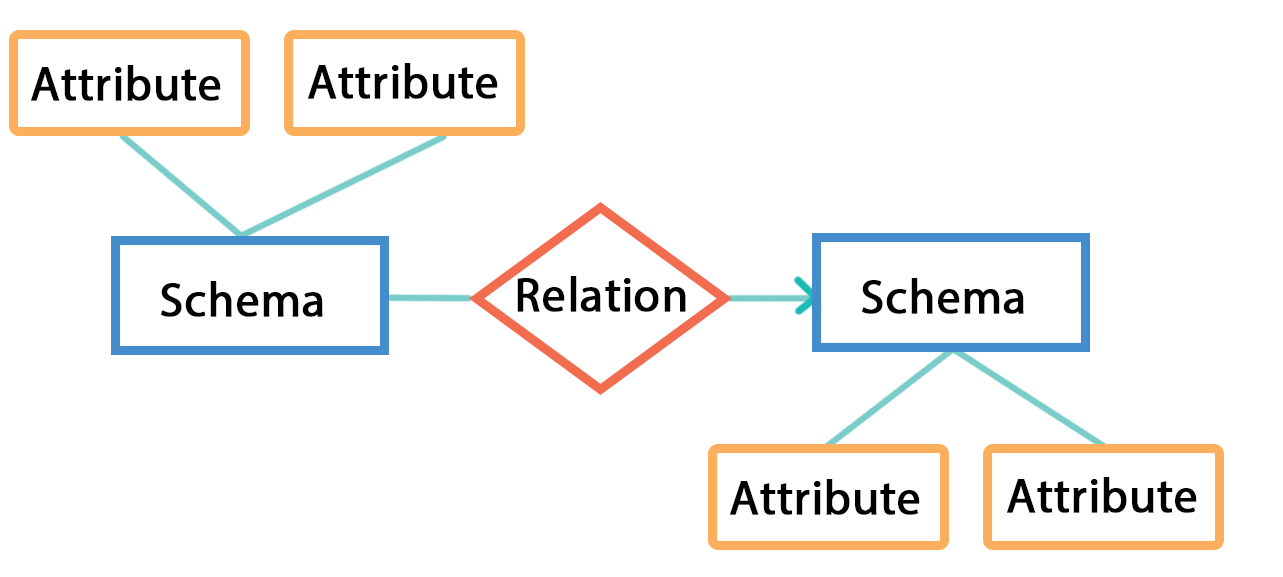
\includegraphics[width=300px]{assets/ERModel.png}
		\end{figure}
		A tuple in the model is called a relationship.\\
		A relation may have mannnny sets attached.\\
		Edges may also have labels, to indicate if two schemas are related in more ways.\\
		A relation may also have attributes, in cases where it makes the most sense. This can also be replaced by a relation more if, many attributes may accour.\\
		Some models like UML does not allow more than a binary relation. To combat this a connecting schema, from which relations can go out to each schema.
		\subsection{Multiplicity of ER models}
				  ER diagrams can also show restrictions, this include the number of relations a schema can have.\\
				  The standard is many-many, this means a relation may involve as many as it wants from both sides.\\
				  Then there is many-one which dictates that, a relation may only be related to one relation. This is indicated by an arrow which points towards the set if which only one can exist.\\
				  There are also one-one which dictates only one relation can relate to another relation. This is indicated by an arrow at both ends of an edge.\\
				  A rounded arrow means exactly one
		\subsection{Subclasses in ER models}
		
		\begin{figure}[h]
			\centering
			\caption{ER model with the button schema being a subclass of top schema.}
			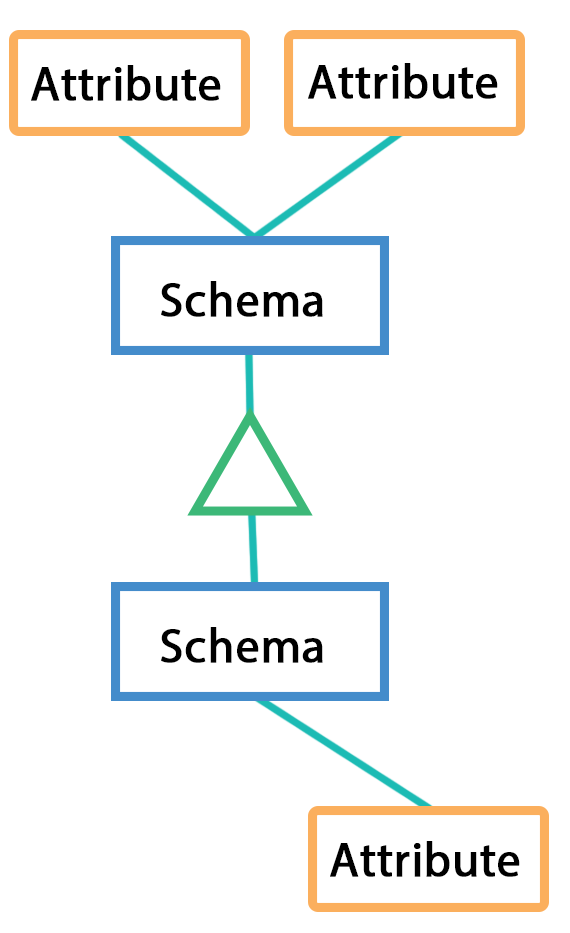
\includegraphics[width=100px]{assets/ERSubclass.png}
		\end{figure}
			A subclass use a isa object to show the subclass relation.\\
			The object is in form of a triangle, where the parent is connected at the top and the subclass at the bottom.\\
			The subclass will then inhert all attributes from the parent and can have new attributes or relations.\\
			A isa object is always one-one, but the arrows are not needed.
		\subsection{Designing a model}
			To create a good model, the model should be simple and not include redundant infomration.\\
			Be of course as faithfull to what it tries to model.\\
			In some cases, a relation may not be the answer. If the the set E:
			\begin{itemize}
						\item Has only arrows entering it.
						\item The only key in E is all attributes.
						\item No relationship involves E more than once
			\end{itemize}
			If all these cases are met, the relation and the set should be removed, and the attributes of E and the relation should be in the related schema.\\

			
		\subsection{Keys in ER models}
		
		\begin{figure}[h]
			\centering
			\caption{ER model with a weak key, where the left schema has two keys its own attribute and the attribute from the right schema}
			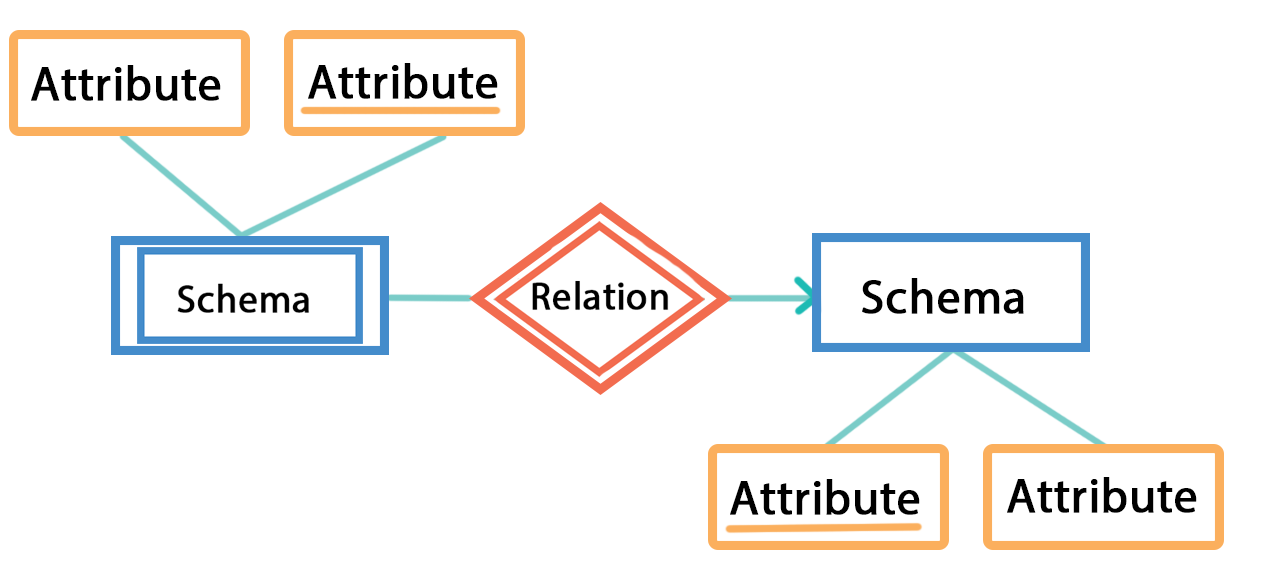
\includegraphics[width=300px]{assets/ERWeak.png}
		\end{figure}
			In ER models keys work like in DBMS.\\
			Here the constraints are that a set must have a key, otherwise it is not a set, which a relation can form.\\
			There may be more than one key, but a primary key must be picked.\\
			With isa's the enitity must have a key which is inherted from the parent.\\
			The key is shown by underlining the key attribute(s).\\
			A weak key is a key from another set.\\
			Weak keys can be valid, in a many-one binary relation which must exist.\\
			In this scenario a key from set F can be used as a weak key for set E.\\
			This is illustrated by the a double rectangle on the set with the weak link and a double border on the relations diamond which provides the weak key.
		\subsection{Constraints}
			A model may also include constraints in the relations.\\
			By using rounded arrows, not only is it many-one relation, it states that at least one set must exists in the relation.\\
			In the case of a restriction on the many-many relation, number critera (Ex, $<10$) is written at the intersect of edge and set and states the minimum.
		\subsection{Converting from ER diagram to DB model}
			To convert it is pretty straight up. The given sets and relations are converted into schemas, with the given attributes.\\
			It may be needed to combine some schemas, this is common if a schema mostly just contains keys, and a many-one is in place.\\
			In this case a big schema can be made, where the relations attributes and the schema with mostly key attributes are added.\\
			When working with weak keys, the key attribute simply is the weak schema, the relation schema and of course the original schema.
			\subsubsection{isa objects}
				To convert isa object there are multiple ways.\\
				The most strightforward way is creating everything as schemas.\\
				Then the keys will connect each schema to the other to obtain all information.\\
				The object oriented approach, makes every possible schema combination according to the isa object.\\
				The null approach creates a schema with all attributes, from every set in the isa. Then null values are made when the object is parent etc.\\
				The null approach makes queries the most simple and fast, but uses more unused space unlike the object orented approach which has only one tuble for every entry with no nulls, but many schemas.
		
				\end{document}
